\section{Pr\'esentation des th\'eorème}



\subsection{Modèle de la simulation sur VM}
\citep{adams2012hitchhiker}
\begin{figure}[h!]
\centering
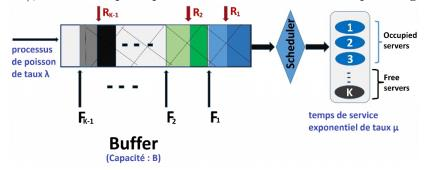
\includegraphics[width=0.70 \textwidth]{photo/modele_vm.jpg}
\caption{le data center avec une file d'attente multi serveur et avec une politique à seuils.}
\label{fig:graphe}
\end{figure}
\\
\noindent Comme le modèle de machines virtuelles décrit par la figure ci dessus,il nous propose que les clients arrivent dans la file d’attente multi-serveur (nous considère que 3 serveurs, 6 serveurs et 12 serveurs à l’évoluation dans la partie de l’étude experimentale), et les serveurs sont activés selon l’occupation du système. Au départ, un seul serveur était activé, puis quand le nombre de clients dépassera $F_{1}$, on activera un deuxième serveur, et jusqu’au seuil $R_{k}-1$ pour activer le k-ème serveur à la fois des désactivation des seuils $R_{1}$, ..., $R_{k}$-1.
\\
\noindent Autrement dit, on contôle le nombre de clients. S’ils dépassent de $R_{1}$ (ou $F_{1}$) on désactive le deuxième serveur, et donc un seul serveur est toujours activé. 
\\
\noindent Dans notre modèle, on définie qu’au départ des processus avec chacune en temps d’inter-arrivée Exponentielles $\frac{1}{\lambda}$ et ceux en temps de service Exponentiel de moyeene $\frac{1}{\mu}$.


\subsection{Chaîne de Markov}

\begin{tikzpicture}[auto,node distance = 2mm,start chain = going right,state/.append style = {thick,  minimum width=2.8em,text width=2.5em,align=center,on chain,fill=red, draw=none,text=black
 },
]

\node (s0)[state]    {$1$};   
\node (s1)[state]    {$2$};  
\node (s2)[state]    {$3$};  
\node (s3)[state]    {$F_{1}-1$};  
\node (s4)[state]    {$F_{1}$};     
\node (s5)[state]    {$r-1$}; 
\node (s6)[state]    {$r$}; 
\node (s7)[state]    {$B-1$}; 
\node (s8)[state]    {$B$}; 

\draw[->] (s0) edge[bend left] node (a1) {$\lambda$} (s1)
          (s1) edge[bend left] node (b1) {$\mu$} (s0)
          (s1) edge[bend left] node (a2) {$\lambda$} (s2)
          (s2) edge[bend left] node (b2) {$\mu$} (s1)
          (s3) edge[bend left] node (a3) {$\lambda$} (s4)
          (s4) edge[bend left] node (b3) {2*$\mu$} (s3);
\node[node distance=0.005cm,right=of s2] {$\bullet$ }; 

\draw[->] (s5) edge[bend left] node (a4) {$\lambda$} (s6)
          (s6) edge[bend left] node (b4) {$r$*$\mu$} (s5);
\node[node distance=0.005cm,right=of s4] {$\bullet$ }; 

\draw[->] (s7) edge[bend left] node (a5) {$\lambda$} (s8)
          (s8) edge[bend left] node (b5) {$r$*$\mu$} (s7);
\node[node distance=0.005cm,right=of s6] {$\bullet$ }; 
\end{tikzpicture}
\quad \\
\noindent La chaîne de Markov est une suite de variables aléatoires qui permet de faire la modélisation d’évolution dynamique d’un système aléatoire. On note {0 , 1 , 2 ... , F1-1 , F1 , F1+1 ... r-1 , r , r+1 ... , B-1 , B} la suite des instants de transition des états du système $\left \{X_{n},n\geq 0 \right \}$  dans notre suite. Et donc nous n’évoluons la distribution stationaire qu’au travers de la valeur actuelle. 
\quad \\
\noindent Notre modèle va créer et supprimer dynamiquement une machine virtuelle afin de faire l’évoluation. Nous develpons une fonction récursive pour obtenir les probabilités d’état stable du système. Et chaque probabilité est obtenu par la multiplication de P0 par la matrice A.
\quad \\
\noindent On calcule des versions successives de la distribution ainsi : 

\begin{equation}
    P_{i}= P_{0} *A_{i}
\end{equation}
\noindent  Et à chaque itération, ils respectent toujours: 
\begin{equation}
    \sum_{i=0}^{B} P_{i} *A_{i} = 1
\end{equation}

\noindent Quand considère à cette chaîne, on résume que :
\begin{enumerate}

\item 1 er seuil : $0\leq n\leq F_{1}-1$:
\begin{equation}
    A_{0} = 1 ; 
\end{equation}
\begin{equation}
    A_{1} = \left ( \frac{\lambda }{\mu }\right )^{1} ; \: ......
\end{equation}

\begin{equation}
    A_{F_{1}-1} = \left ( \frac{\lambda }{\mu }\right )^{F_{1}-1} ;
\end{equation}

\item 2 ème seuil : $F_{1}\leq n\leq F_{2}-1$:
\begin{equation}
    A_{F_{1}} = \left ( \frac{\lambda }{2*\mu }\right )^{1}\times A_{F_{1}-1} ;  
\end{equation}
\begin{equation}
    A_{F_{1}+1} = \left ( \frac{\lambda }{2*\mu }\right )^{2}\times A_{F_{1}-1} ; \: ......
\end{equation}
\begin{equation}
    A_{F_{2}-1} = \left ( \frac{\lambda }{\mu }\right )^{F_{2}-1-(F_{1}-1)}\times A_{F_{1}-1} ;
\end{equation}
......
\item n ème seuil (n est égal au nombre des serveurs): $F_{r}\leq n\leq F_{B}$:
\begin{equation}
    A_{F_{r}} = \left ( \frac{\lambda }{r*\mu }\right )^{1}\times A_{F_{r-1}-1} ; \: ......
\end{equation}
\begin{equation}
    A_{F_{B-1}} = \left ( \frac{\lambda }{r*\mu }\right)^{F_{B-1}-1-(F_{r}-1)}\times A_{F_{r-1}-1} ;
\end{equation}
\begin{equation}
    A_{F_{B}} = \left ( \frac{\lambda }{r*\mu }\right)^{F_{B}-1-(F_{r}-1)}\times A_{F_{r-1}-1} ;
\end{equation}
\end{enumerate}


\subsection{Algorithmique de calculer $A_{0}$...$A_{B}$}

\noindent Pour initialiser la matrice des seuils, on mise la distribution du nombre des états dans chacune. Et la capacité de file d'attente est initialisé à B. Dans ce cas là, si nous enregistrons tous les états de 0 à B , le nombre total des éléments posés dans la matrice est égal à B+1 (états). 
\quad \\
\noindent L’algorithme qu’on aurait dût implémenter est le suivant :
\begin{algorithm}
\caption{Calculer des valeurs de $A_{0}$...$A_{B}$}


\label{alg:Calculer des valeurs de A}
\begin{algorithmic}
\STATE {$function mat\left [ \right ] = Calculer\:A(index,\lambda,\mu\:tmp,pre)\{$} 
\STATE set $i=1$ 
\STATE set $tmp=0$ 

\REPEAT 
\IF {$index < Nb\:serveur$}
\IF {$index == 0$}
\FOR{$i=1$ to $seuils[index]$}
\STATE $tmp=\left ( \frac{\lambda }{\mu }\right )^{i-1-0}\times pre;$ 
\STATE $sum\:A=sum\:A + tmp;$ 
\STATE $mat\:A[]=ajout\:matrice(mat,tmp,pos+i-1);$ 
\ENDFOR

\ELSE
\FOR{$i=1$ to $seuils[index]$}
\STATE $tmp=\left ( \frac{\lambda }{\mu }\right )^{seuils[index-1]+i-1)-(seuils[index-1]-1)}\times pre;$ 
\STATE $sum\:A=sum\:A + tmp;$ 
\STATE $mat\:A[]=ajout\:matrice(mat,tmp,pos+i-1);$ 
\ENDFOR
\ENDIF

\STATE $pos = pos+seuils[index];$ 
\STATE $pre = tmp;$ 
\STATE $index++;$ 
\STATE $Calculer\:A(index,\lambda,\mu\:tmp + \mu,pre);$ 



\ELSE
\STATE $P_{0}=\frac{1}{sum\:A};$
\STATE $return\:\: mat\:A[];$
\ENDIF

\UNTIL{$index < Nb\:serveur$ }\\\}
\end{algorithmic}
\end{algorithm}

\subsection{Les formules d'analyser le système}
\noindent En fonction du nombre total de VMs, de la capacité du système et des seuils, nous analysons notre système avec des résultats calculés par l'algorithmique . Pour se faire: 
\begin{enumerate}
\item Calculer $P_{0}$ :
\begin{equation}
P_{0} + P_{1} + ... + P_{F_{1}-1} + P_{F_{1}} + ... P_{B} = 1
\end{equation} \\
\begin{equation}
P_{0} \times \left (  A_{0} + A_{1} + ... + A_{F_{1}-1} + A_{F_{1}} + ... A_{B} \right ) = 1 
\end{equation}\\
\begin{equation}
P_{0}=\frac{1}{\sum_{i=0}^{B} A_{i}}
\end{equation}

\item Probabilit\'e de blocage est égale à la probabilité qui se trouve dans l'état B:
\begin{equation}
    Pr = 1-\sum_{i=0}^{B-1}P_{i} = P_{B} = \left ( \frac{\lambda}{\mu}\right )^{B-1-\left ( r-1\right )}\times \cdot \cdot \cdot  \left ( \frac{\lambda}{\mu}\right )^{F_{2}-1-\left ( F_{1}-1\right )}\times \left ( \frac{\lambda}{\mu}\right )^{F_{1}-1}\times P_{0}
\end{equation}
\item Nombre moyen de requêts :
\citep{adams2015hitchhiker}
\begin{equation}
Nb\: moyen\: de\: requetes =\sum_{i=0}^{B}\left (i \times P_{i} \right ) 
\end{equation} 

\item Nous considèrons que la distribution selon des probabilités à chaque VM comme par exemple (6 clients arrivent dans 3 VMs):

\begin{center}
\begin{tabular}{ |c|c|c| } 
 \hline
 VM1 & VM2 & VM3 \\ 
 \hline
 2 états & 3 états & 2 états\\
 \hline
 $1 \times P_{0} + 1 \times P_{1} $&$ 2 \times P_{2} + 2 \times P_{3}+ 2 \times P_{4}$ & $ 3 \times P_{5}+3 \times P_{6}$ \\ 
 \hline
\end{tabular}
\end{center}

\noindent Nombre de machine virtuelles en fonctionnement :
\begin{equation}
Nb\:de\: vm = \sum_{i=1}^{nb\: de\: serveurs}\left (i\times \sum_{j=F_{\kappa}}^{F_{\kappa +1}-1}P_{j} \right )
\end{equation}
\noindent  ( Chaque VM fait lancer dans l’intervalle de état : $\left [ F_{\kappa},F_{\kappa +1}-1 \right ]$. )
\end{enumerate}

















 



